\documentclass[journal]{IEEEtran}
\usepackage{amsmath,amsfonts}
\usepackage{algorithmic}
\usepackage{algorithm}
\usepackage{array}
\usepackage[caption=false,font=normalsize,labelfont=sf,textfont=sf]{subfig}
\usepackage{textcomp}
\usepackage{stfloats}
\usepackage{url}
\usepackage{verbatim}
\usepackage{graphicx}
\usepackage{cite}
\usepackage{booktabs}
\usepackage[hidelinks]{hyperref}

\usepackage{xcolor}
\usepackage{soul}

\begin{document}

\title{Transfer learning between Sentinel-1 acquisition modes enhances \\ the few-shot segmentation of natural oil slicks in the Arctic}

\author{Julien Vadnais,~\IEEEmembership{Graduate Student Member,~IEEE, }Benjamin Aubrey Robson, Christian Haug Eide, Rune Mattingsdal, Malin Johansson
        % <-this % stops a space
\thanks{Manuscript received March 31, 2025. This research was carried out in the context of the InFluSe project (Research Council of Norway Project 353044).}

% grouped affiliations
\thanks{Julien Vadnais, Benjamin Aubrey Robson, and Christian Haug Eide are with the Department of Earth Science, University of Bergen, 5020 Bergen, Norway.
Rune Mattingsdal is with the Norwegian Offshore Directorate, 9406 Harstad, Norway.
Malin Johansson is with the Department of Physics and Technology, The Arctic University of Norway, 9037 Tromsø, Norway.} 

%separate affilations
% \thanks{Julien Vadnais, Benjamin Aubrey Robson, and Christian Haug Eide are with the Department of Earth Science, University of Bergen, 5020 Bergen, Norway.}
% \thanks{Rune Mattingsdal is with the Norwegian Offshore Directorate, 9406 Harstad, Norway.}
% \thanks{Malin Johansson is with the Department of Physics and Technology, The Arctic University of Norway, 9037 Tromsø, Norway.}
\thanks{Corresponding author email address: julien.vadnais@uib.no. All data and code used in this study is accessible on the GitHub repository \url{https://github.com/julvad/transfer_learning_S1_slicks_arctic}}
 
\thanks{}% <-this % stops a space
}

% The paper headers
\markboth{\LaTeX\ PDF, IEEE GEOSCIENCE AND REMOTE SENSING LETTERS,~Vol.~14, No.~8, March~2025}%
{Shell \MakeLowercase{\textit{et al.}}: A Sample Article Using IEEEtran.cls for IEEE Journals}

\IEEEpubid{\copyright This work is licensed under CC BY 4.0.}
% Remember, if you use this you must call \IEEEpubidadjcol in the second column for its text to clear the IEEEpubid mark.

\maketitle

\begin{abstract} 
    Natural seepage is a significant contributor to marine hydrocarbon inputs. Remote and intermittent seeps are difficult to monitor in the field, yet oil slicks can be observed from spaceborne 
    synthetic aperture radar (SAR) due to differences in their backscatter,
    creating potential for automatic mapping. In mapping tasks such as segmentation, deep learning models excel, whilst needing large amounts of labeled images.
    To deal with scarcity of labeled images, transfer learning is an approach 
    commonly used in computer vision, yet still underutilized in remote sensing. In the case of oil slicks, differences between Sentinel-1 acquisition modes—such as the 
    interferometric wide (IW) in the North Sea and extra-wide (EW) in the Arctic—complicate direct model transfer.
    Here, we present a use-case where transfer learning enhances the segmentation of natural oil slicks. We used labeled slicks in IW images in the North Sea to pretrain a series of DeepLabv3 and SAM models. 
    These models were then fine-tuned on EW-labeled slicks from two documented Arctic seeps on which we have only limited observations. Our results show clear evidence that transfer learning improves few-shot 
    segmentation, even in challenging images with slick look-alikes. Overall, few studies have addressed transfer learning between SAR acquisition modes, and this work contributes to 
    better monitoring poorly understood or yet undiscovered natural oil seeps. 
\end{abstract}

\begin{IEEEkeywords}
    Natural seepage, oil slicks, SAR, deep learning, transfer learning, segmentation, DeepLab, SAM.
\end{IEEEkeywords}

\section{Introduction}
\IEEEPARstart{N}{atural} seepage is a significant contributor of oil entering marine environments \cite{kvenvoldenNaturalSeepageCrude2003}, yet the data required to update quantitative
estimates of its global scale remain insufficient, especially outside of the United States continental shelf \cite{nationalacademiesofsciencesengineeringandmedicineOilSeaIV2022}. Because of difficulties 
in monitoring remote offshore areas and keeping continuous observations, data scarcity has restrained our possibilities of studying the ecosystem contribution and the behavior of natural hydrocarbon seeps. 
Synthetic aperture radar (SAR) is well suited to this task due to its capacity to operate in any lighting conditions, and its fine spatial resolution for its wide swath coverage. 
Oil slicks are visible in SAR because they return lower backscatter compared to surrounding waters, due to oil reducing sea roughness \cite{brekkeSAROilSpill2020,fingasReviewOilSpill2018,alpersOilsSurfactants2004}.
In precise terms, SAR's capacity for detecting a slick relies on the damping ratio, the contrast in radar backscatter between slick and oil-free pixels \cite{hovlandSlickDetectionSAR1994,
quigleyInvestigationDampingRatio2023}.

Many previous works have attempted to make use of the damping ratio for automatizing marine oil detection, with varying results. They face a common challenge which has been an ongoing topic of research for over 
three decades: the presence of oil slicks look-alikes including ocean eddies, biogenic slicks and newly-formed ice \cite{johanssonCanMineralOil2020,hovlandSlickDetectionSAR1994,alpersOilsSurfactants2004,
alpersOilSpillDetection2017,espedalSatelliteDetectionNatural1996}. 
When trained with a large number of labeled examples, deep learning models, currently the benchmark in computer vision, can capture complex shape- and texture-related features for image classification or 
segmentation tasks \cite{goodfellowDeepLearning2016}. When trained with a limited sample size, however, these models struggle to extract more abstract, higher-level features
\cite{bengioDeepLearningRepresentations2012}. The issue of limited data is exacerbated in the case of natural slicks mapping because of limited visibility. 
Not only will slicks only last a few hours on the surface \cite{jatiaultMonitoringNaturalOil2017,daneshgaraslHindcastModelingOil2017,oreillyDistributionMagnitudeVariability2022}, 
their visibility also depend on a specific window of surface wind conditions, outside of which the sea either has too many or too few capillary waves for a discriminative 
damping ratio \cite{quigleyInvestigationDampingRatio2023,sausDetectionDelineationProduced2021,gadeImagingBiogenicAnthropogenic1998}. 
\IEEEpubidadjcol  
Slick events are also highly intermittent. Seepage rates vary considerably across both monthly and yearly timescales, most active slicks having an occurence rate below 10\% 
\cite{jatiaultNaturalOilSeep2024,oreillyDistributionMagnitudeVariability2022}. Some seeps remain dormant for several months or even years before emitting oil again. Only half of the seeps show activity at any time 
\cite{jatiaultMonitoringNaturalOil2017,garcia-pinedaRemotesensingEvaluationGeophysical2010}, and dormant seeps might be underestimated considering they are less likely to be discovered.

In this paper, we assess the potential of transfer learning for enhancing the automatic mapping of natural slicks. Transfer learning, or deep transfer learning in the case of deep learning, aims at 
transferring valuable and generalizable features from one model to another, where the contexts are similar but the target distributions differ \cite{goodfellowDeepLearning2016}. 
We pretrained two image segmentation models using oil slicks mapped in Sentinel-1 images over the North Sea. These models were then fine-tuned on two known seeps in the Arctic, for which we have only 
limited observations. In the Arctic, Sentinel-1 scenes are mostly acquired in the extra-wide (EW) mode at a 25-meter resolution with dual HH/HV polarization. However, elsewhere, oil slick mapping with 
Sentinel-1 more commonly uses the interferometric-wide (IW) mode at a 10-meter resolution with the VV polarization.
%Over the Arctic, Sentinel-1 scenes are mostly acquired in the 25-m resolution extra-wide (EW) mode with a dual HH/HV polarization, whereas oil slick mapping with Sentinel-1 more often use the 
%interferometric-wide (IW) mode, of 10-m pixel resolution with a dual VV/VH polarization. 
Little work, if any, has so far addressed transfer learning between SAR acquisition modes, and we believe natural oil slicks make a 
prime example of a real-life application of deep-learning mapping with few labeled data. 

\section{Data and methods}
\subsection{Data}
Traditional transfer learning in remote sensing imply that the \textit{target domain} $\mathit{D}_T$ and the \textit{source domain} $\mathit{D}_S$ have similar probability distributions 
between a common feature vector $\mathbf{x_i}$ and a common label $\mathbf{y_i}$ \cite{tuiaDomainAdaptationClassification2016}. Deep transfer learning is more robust to distribution shifts 
and can even handle different target classes, yet this often requires training on massive datasets (e.g. \cite{heDeepResidualLearning2015,kirillovSegmentAnything2023}). 
Our approach is rather a domain-targeted form of deep transfer learning, with a smaller $\mathit{D}_S$ dataset, but closer to the $\mathit{D}_T$. Let's introduce those two domains.

Researchers recently documented two seeps in the Norwegian waters. First, Panieri et al. \cite{panieriArcticNaturalOil2024} investigated an intermittent seep offshore Prins Karls Forland 
(10.42°E, 78.49°N), west of the Svalbard archipelago. At this location, we manually delineated oil slicks extending from a common seeping point, in 70 images between 2015 and 2024.
Second, Serov et al. \cite{serovWidespreadNaturalMethane2023} (but see also Ivanov et al. \cite{ivanovSearchDetectionNatural2020}) gave extensive evidence of a wide seepage area in the Barents Sea. 
This area is part of the Sentralbanken high, a geological structure with prospective hydrocarbon potential, although it remains largely unexplored \cite{lundschienNorthBarentsComposite2025}. 
There (31.33-32.37°E, 75.15°N-75.35°N), we mapped 250 natural slicks in 88 images between 2015 and 2020.
At those two locations, labeled samples from the horizontal co-polarization (HH) band of Sentinel-1 EW images make the $\mathit{D}_T$ (Fig. \ref{figure1}a, \ref{figure1}b). 
At lower latitudes, oil slicks of various kinds can be observed in the North Sea, an hydrocarbon-rich and seepage-active region \cite{hovlandChapter2Focus1988}. 
With the same procedure, we mapped over 1700 slicks, this time using the vertical co-polarization (VV) band of 463 Sentinel-1 IW images. Here, labeled samples in the North Sea make the $\mathit{D}_S$ (Fig. \ref{figure1}c).
Only the co-polarization bands were used, considering their oil-discrimination capacity \cite{kudryavtsevDualCoPolarizedSAR2013,johanssonMultifrequencyPolarimetricSAR2017,brekkeSAROilSpill2020}.
Since a slick can be split in more than one part if its extent is not fully connected, we give slick numbers in Table \ref{table1} as approximations only.
\begin{figure}[!t]
    \centering
    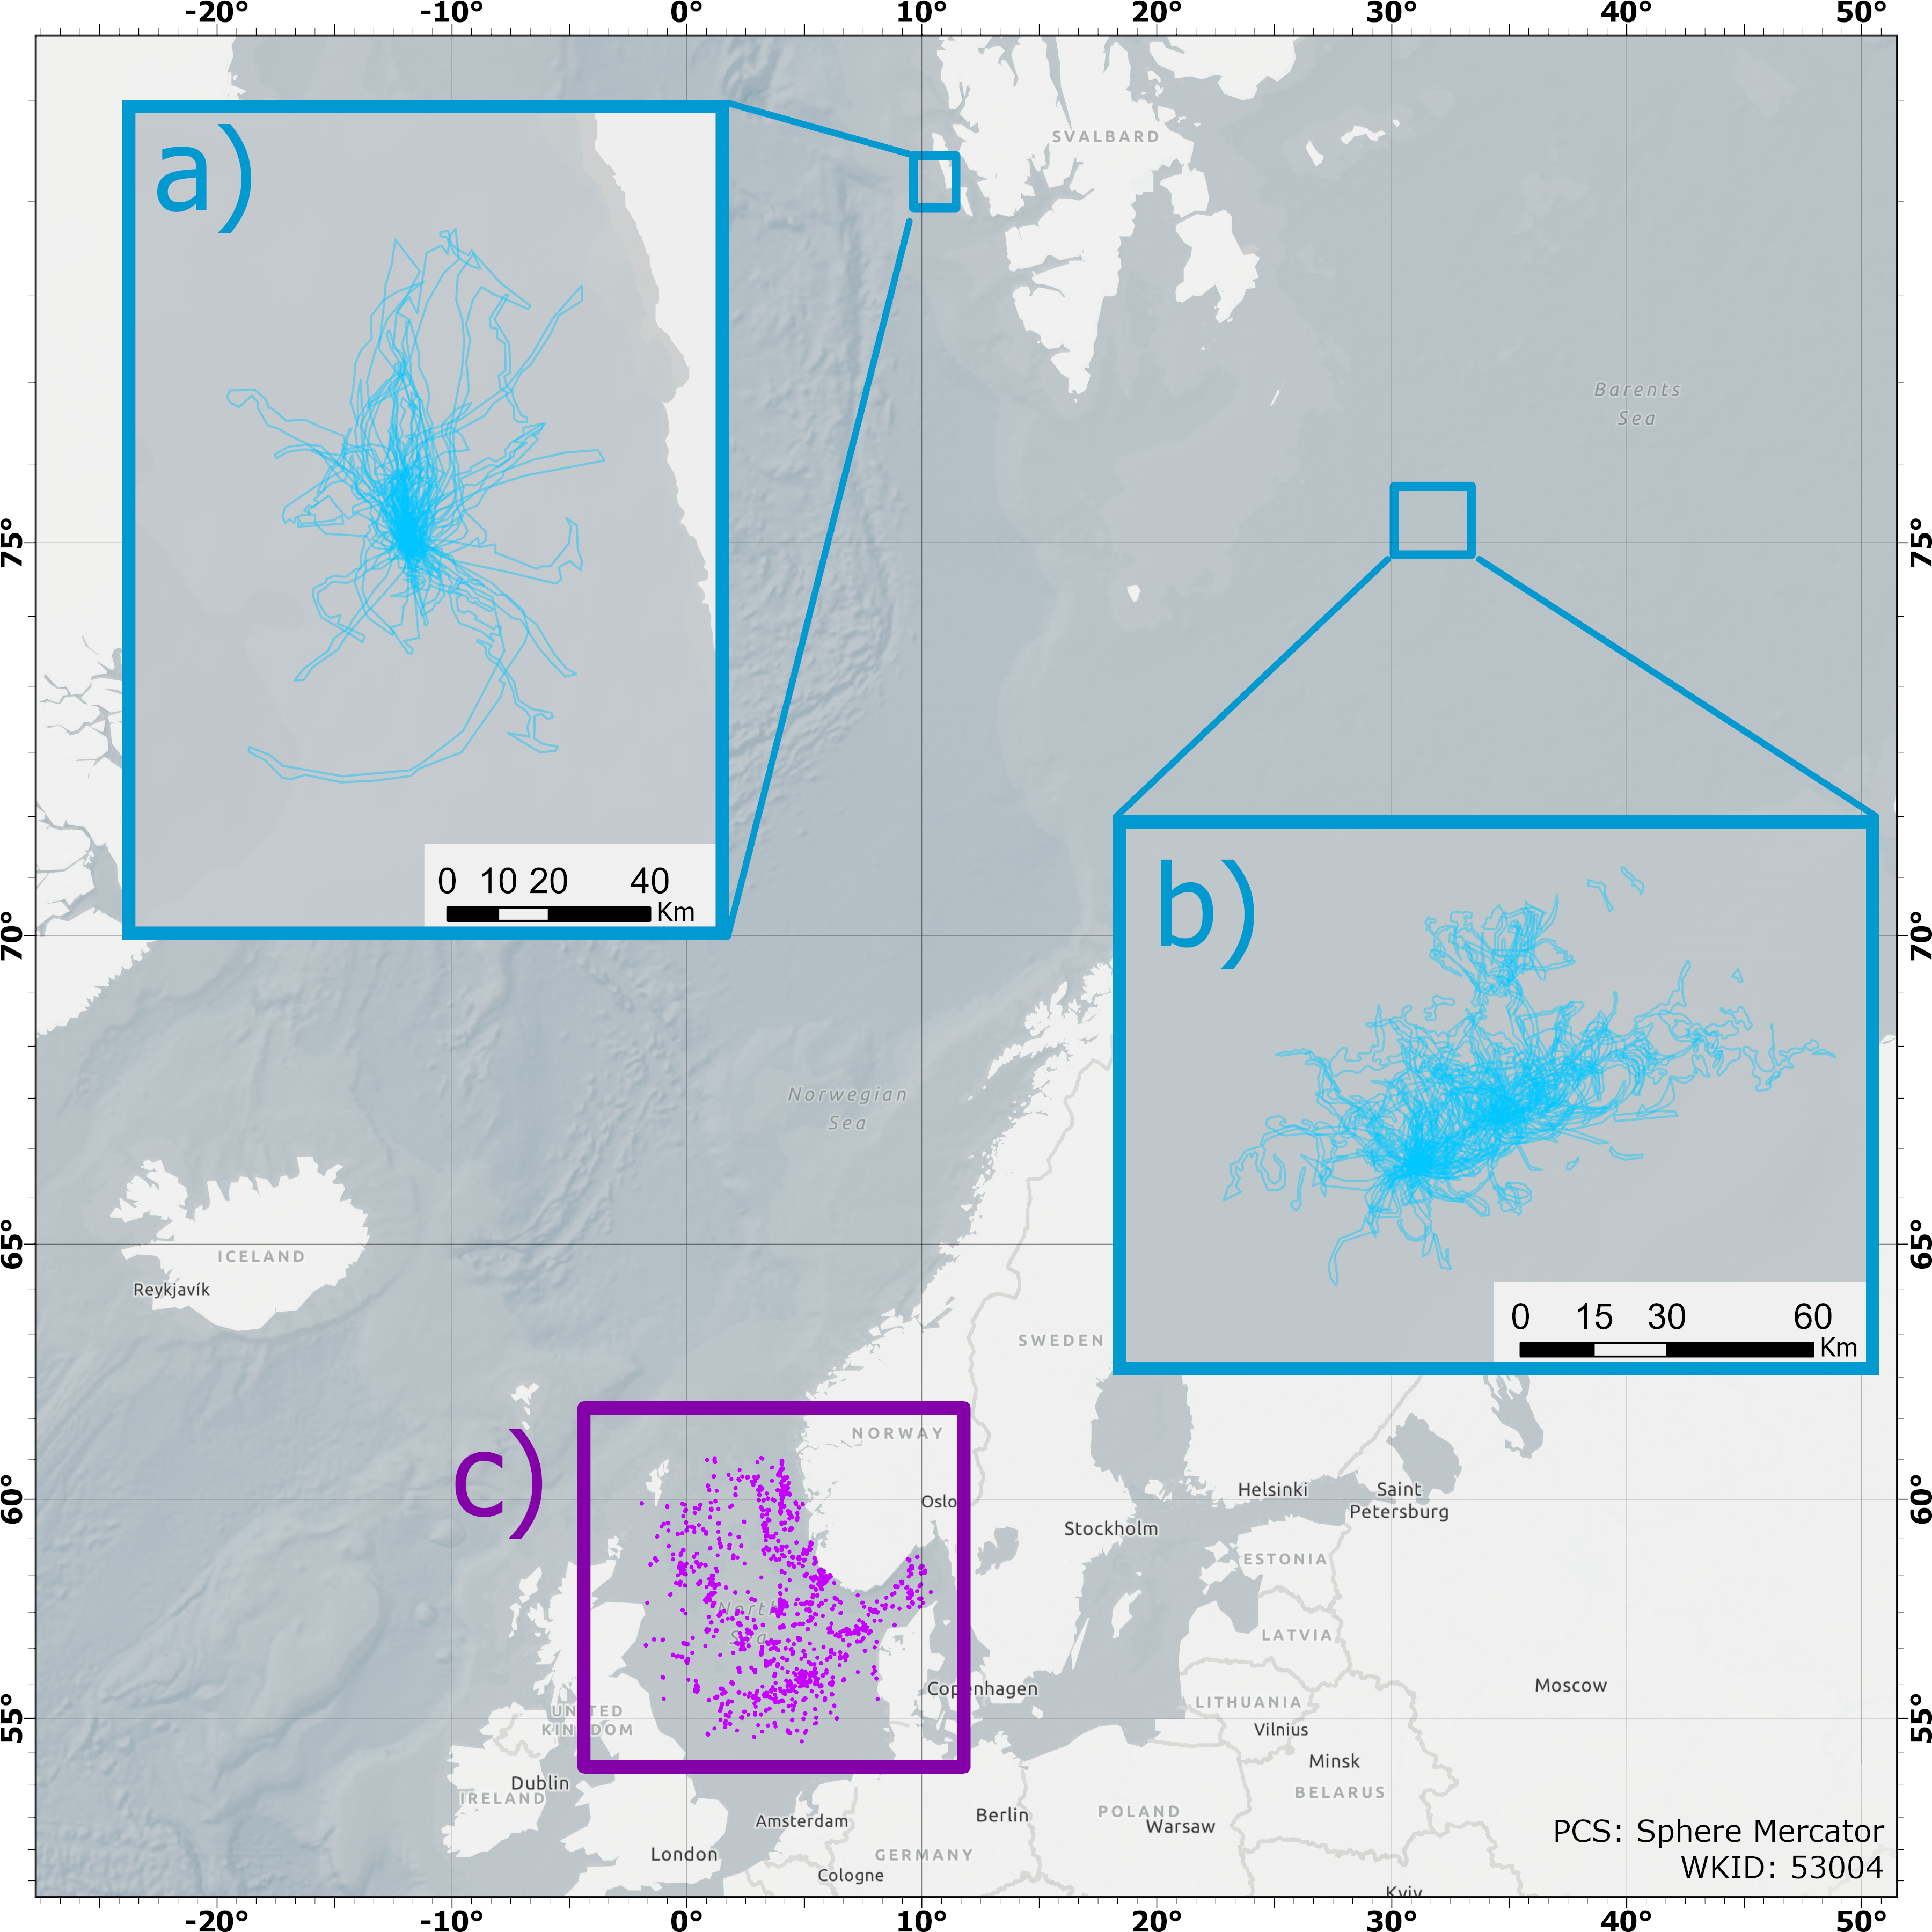
\includegraphics[width=3.3in]{figures/layout2_grids.png} %3.3=left 3.5=right
    \caption{a) Target domain \( \mathit{D}_T \): Mapped slicks offshore Prins Karls Forland, Svalbard \quad b) Target domain \( \mathit{D}_T \): Mapped slicks in Sentralbanken high, Barents Sea \quad 
    c) Source domain \( \mathit{D}_S \): Mapped slicks in the North Sea}
    \label{figure1}
\end{figure}
\begin{table}[!t]
    \caption{Labeled Slicks in the Source and Target Domains}
    \label{table1}
    \centering
    \begin{tabular}{lcc|cc}
        \toprule
        & \multicolumn{2}{c}{\textbf{Source domain}} & \multicolumn{2}{c}{\textbf{Target domain}} \\
        \cmidrule(lr){2-3} \cmidrule(lr){4-5}
        \textbf{Sentinel-1 mode/pol.} & \multicolumn{2}{c}{IW / VV} & \multicolumn{2}{c}{EW / HH} \\
        \midrule
        \textbf{Area} & \multicolumn{2}{c}{North Sea} & Svalbard & Barents Sea \\
        \textbf{Number of images} & \multicolumn{2}{c}{463} & 70 & 88 \\
        \textbf{Period} & \multicolumn{2}{c}{2017-2021} & 2015-2024 & 2015-2020 \\
        \textbf{Number of slicks} & \multicolumn{2}{c}{$\sim 1723$} & $\sim 81$ & $\sim 250$ \\
        \bottomrule
    \end{tabular}
\end{table}

Transfer learning of remote sensing imagery needs data alignement \cite{tuiaDomainAdaptationClassification2016}. To deal with shape distorsion, particularly at higher latitudes, we reprojected 
all Sentinel-1 scenes into their corresponding UTM zone. This corresponds to the 31N zone for the North Sea, the 32N zone at Prins Karls Forland, and the 36N zone at Sentralbanken high. 
Because the pixel spacing resolution of EW scenes is 25 m compared to 10 m for IW scenes, we ran a bilinear interpolation to align spatial resolutions. A bilinear interpolation is 
generally preferred when working with continuous raster values such as the SAR backscatter intensity \cite{schowengerdtRemoteSensingModels2006}. In the $\mathit{D}_T$, 30 out of the 158 annotated Sentinel-1 EW HH scenes were retained for the test 
split—about 19\%—and 10\% of the training samples were used for validation. We extracted four combinations of square raster tiles, using a tile width of either 256 or 512 pixels, and either downsampling 
resolution to 25 m or upsampling to 10 m. Contrast normalization is another important preprocessing step, which needs to be robust to outliers\cite{goodfellowDeepLearning2016,schowengerdtRemoteSensingModels2006}. 
Here, we applied a linear stretch of two standard deviations on clipped tiles, normalizing values over the 8 bit range (0,255):
\begin{equation}
    X' = \frac{X - \mu }{2 \cdot \sigma} \cdot 255
\end{equation}
in which \( X' \) is the new value of image pixels \( X \), using the mean \( \mu \) and the standard deviation \( \sigma \) of the image.

\subsection{Methods}
We pretrained two deep learning models: DeepLabv3 and the Segment Anything Model (SAM). DeepLabv3 is a convolutional neural network architecture for semantic segmentation which uses atrous convolutions 
and introduced atrous spatial pooling layers \cite{chenDeepLabSemanticImage2018}. It is considered state-of-the-art in many fields of application including remote sensing \cite{tuiaDeepLearningbasedSemantic2021}. 
SAM is a novel zero-shot learning vision transformer for image segmentation \cite{kirillovSegmentAnything2023}. While SAM itself does not assign classes, the SamLoRA variation extends its 
use by adding trainable classification layers to SAM's mask encoder \cite{esriFinetuneSegmentAnything2025}. Data augmentation was generated in the form of a 30° rotation, brightness and contrast shifts, 
soft zooms and croppings. We trained with two backbones to see if a deep or a shallow model would perform best. For DeepLabv3, we used the ResNet-50 and ResNet-101 backbones \cite{heDeepResidualLearning2015}; 
ViT-B and ViT-L checkpoints for SAM \cite{kirillovSegmentAnything2023}. The learning rate was determined from a pretraining learning curve \cite{smithCyclicalLearningRates2017,howardFastaiLayeredAPI2020}. 
We used a training batch size of 64 for the 256x256 tiles, and 16 for the 512x512 tiles. 

Model inference was performed in Python using ArcPy and PyTorch, with a RTX 4500 Ada Generation GPU.
We first experimented training with a weighted binary cross-entropy loss function, defined by:
\begin{equation}
    L_\textit{CE} = -\frac{w}{N} \sum_{i=1}^{N} \left[ y_i \log(\hat{y}_i) + (1 - y_i) \log(1 - \hat{y}_i) \right]
\end{equation}
Here, \( y_i \) represents the ground truth label (0: water; 1: slick) and \( \hat{y_i}  \) is the softmax predicted value of the \( i \)-th pixel. This function introduces \( w \), a weight parameter 
calculated as a scalar inversely proportional to slick pixel frequency\cite{azadLossFunctionsEra2023}. To further handle the frequency imbalance between oil and water pixels, 
we added a term based on slick class Dice loss \( (L_\text{Dice}) \) from \cite{milletariVNetFullyConvolutional2016}, resulting the Dice-weighted loss function:
\begin{figure*}[!t]
    \centering
    \subfloat[]{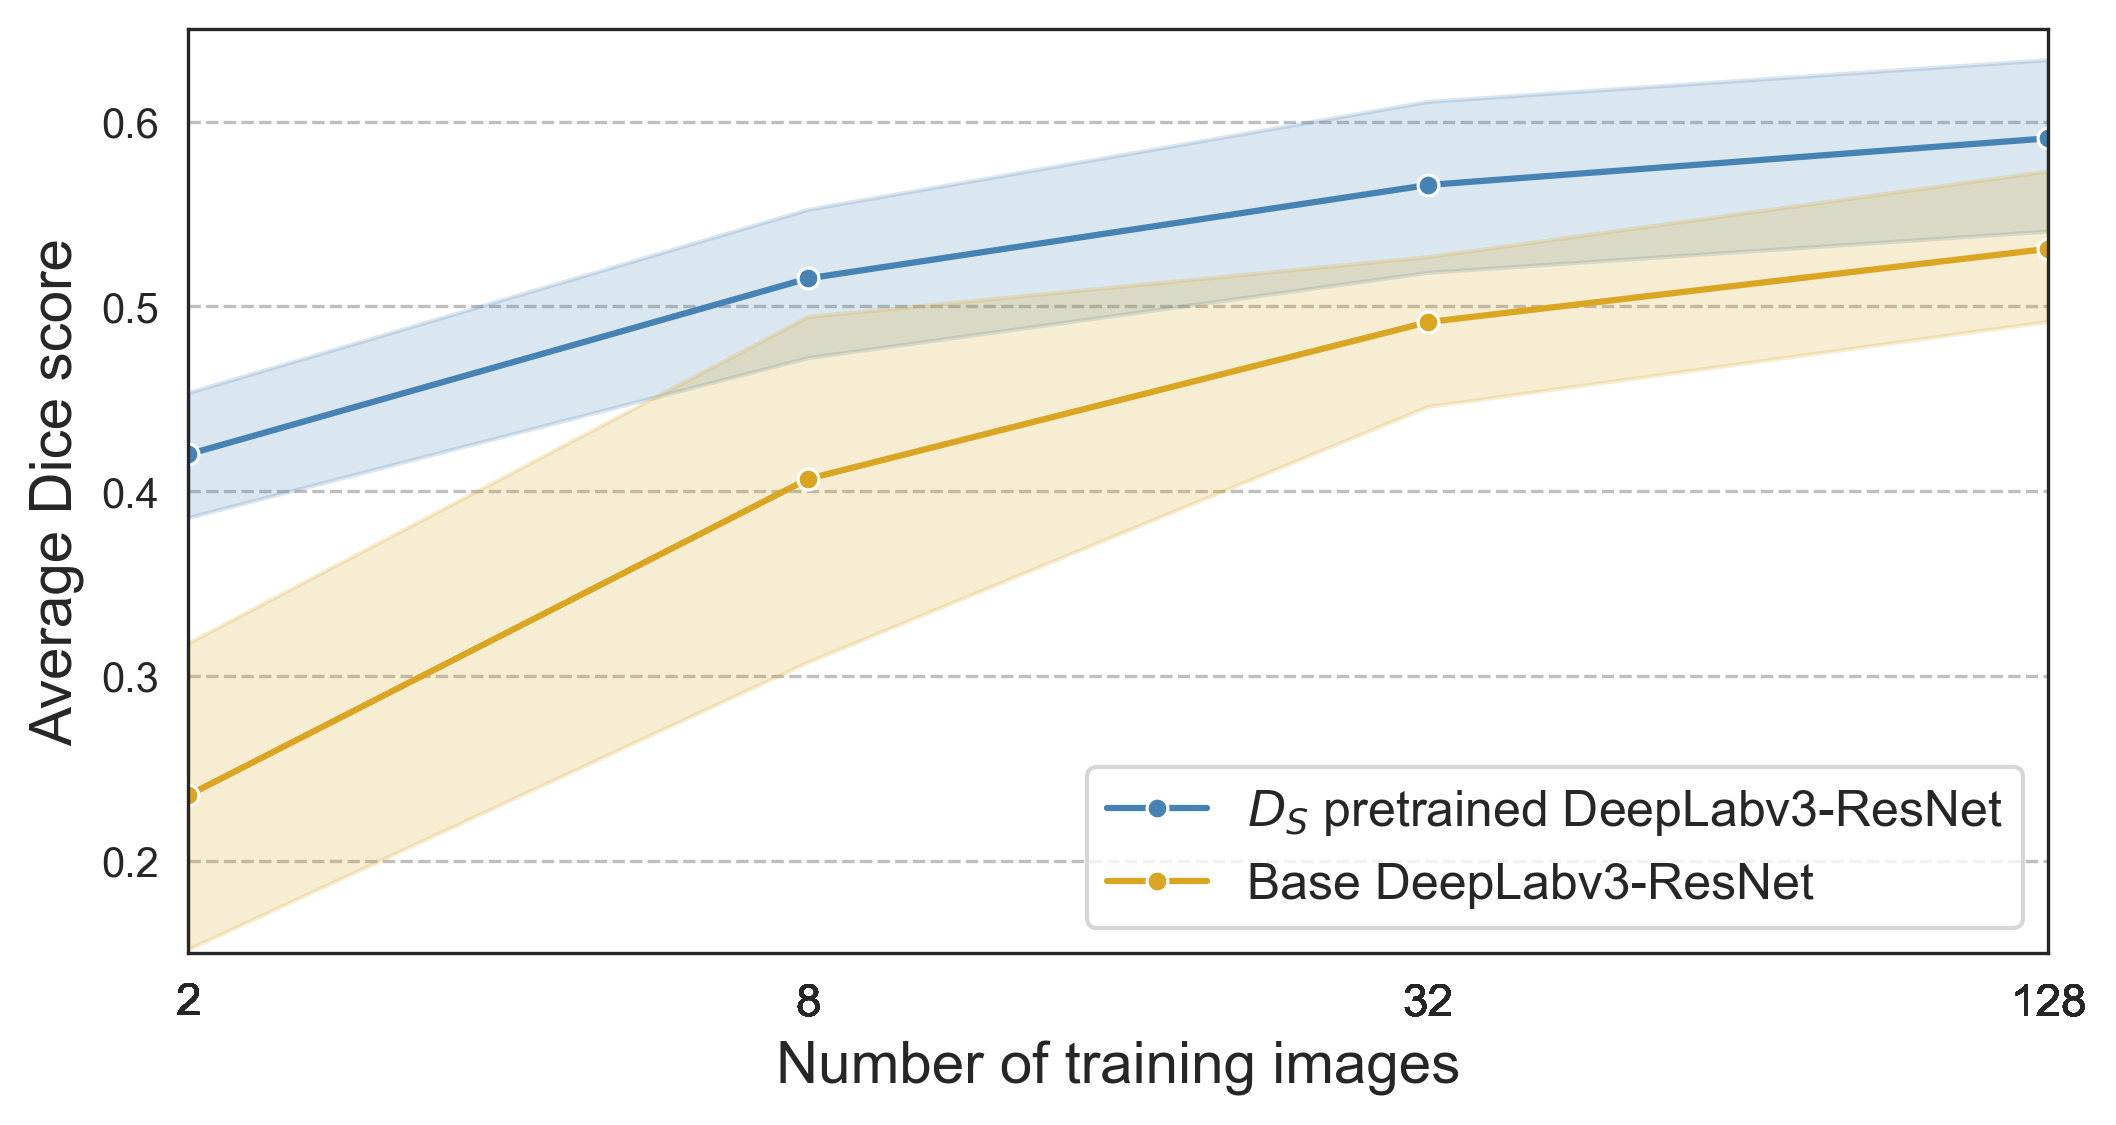
\includegraphics[width=3.18in]{figures/deeplab_dice_temp.png}%
    \label{fig2-1}}
    \hfil
    \subfloat[]{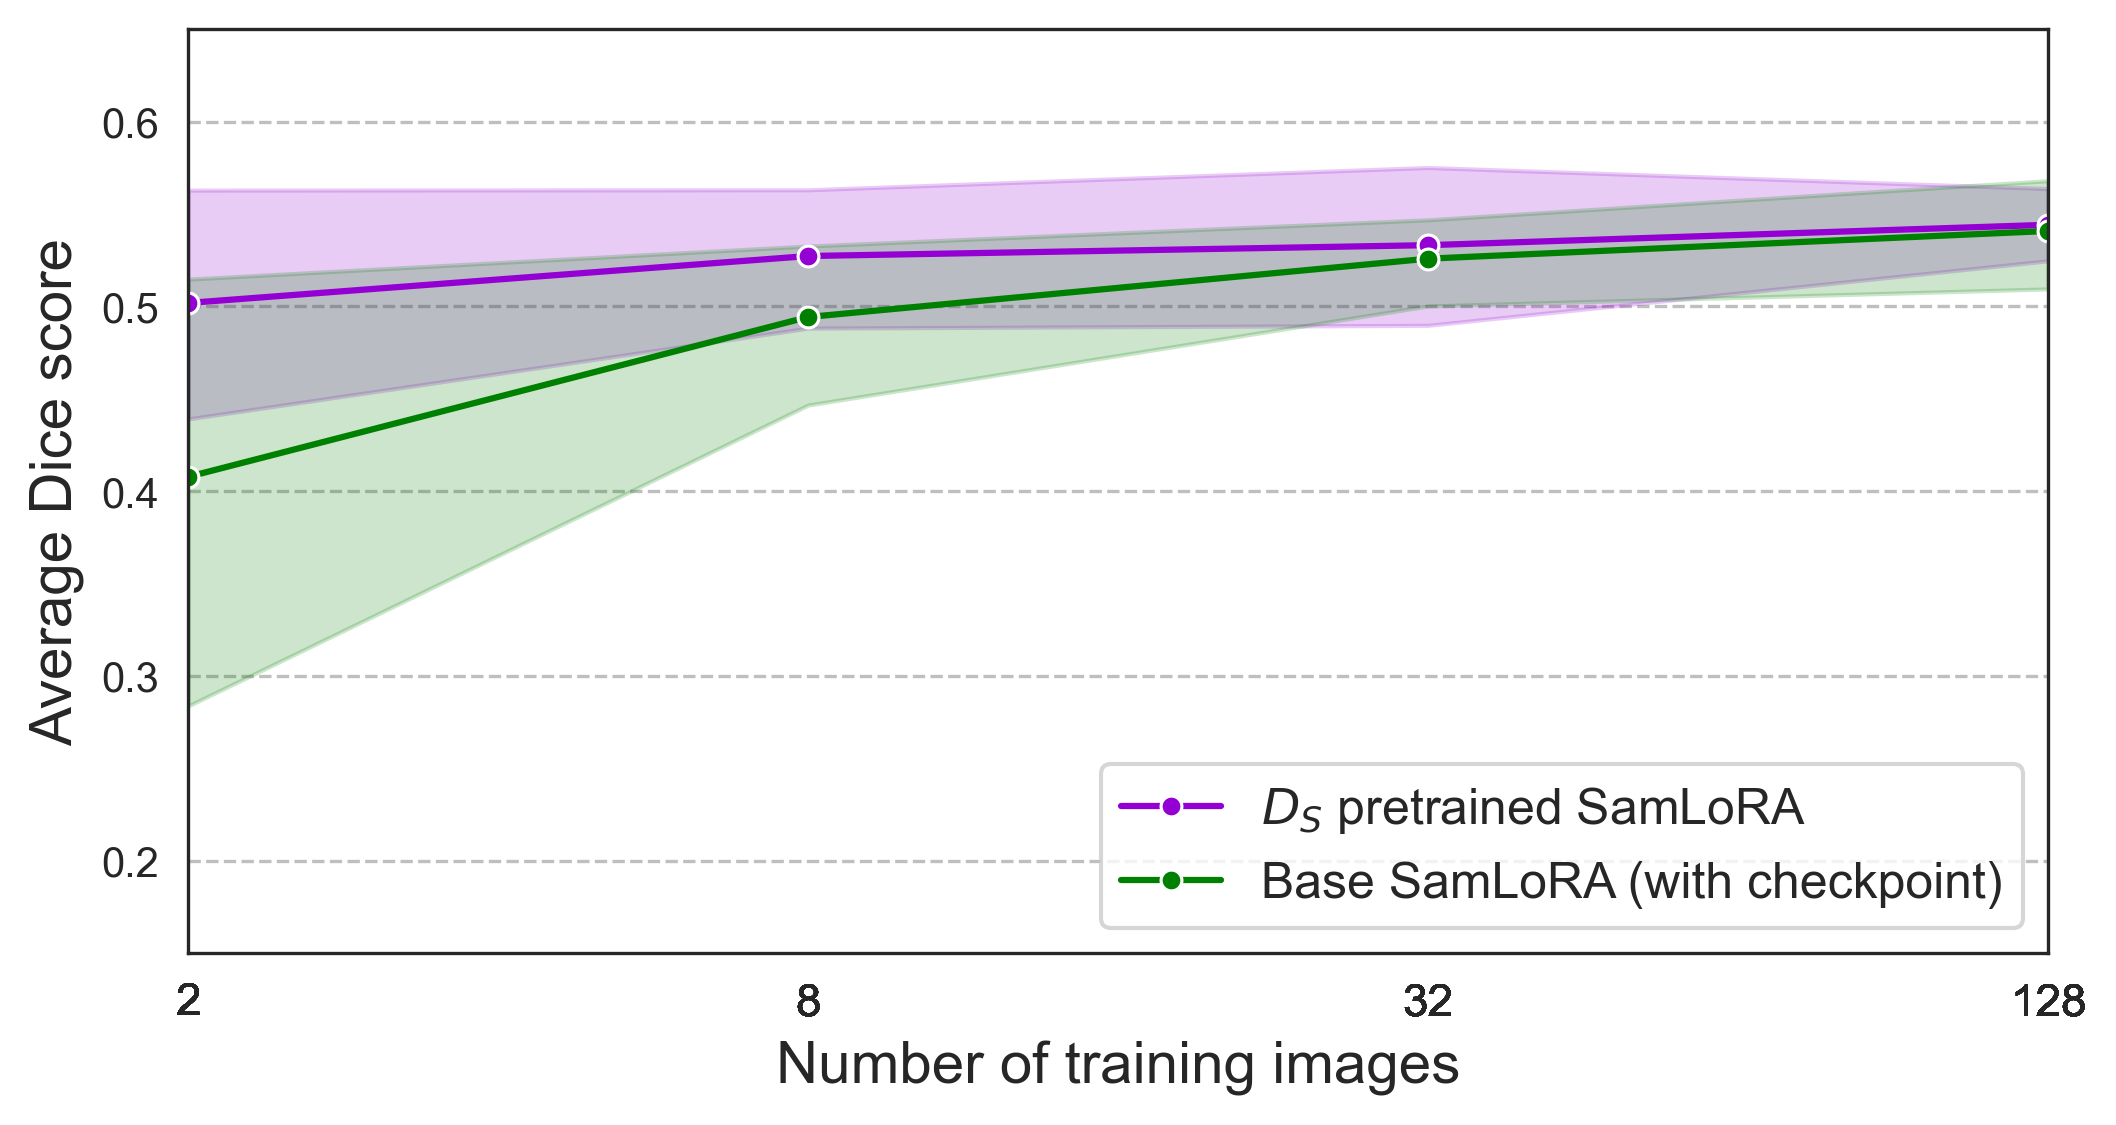
\includegraphics[width=3.18in]{figures/samlora_dice_temp.png}%
    \label{fig2-2}}
    \caption{Average test-set Dice score with 95\% statistical interval, depending on the number of training images. \quad (a) DeepLabv3 \quad (b) SamLoRA }
    \label{figure2}
\end{figure*}
% This gives a simplified version of the Combo loss from \cite{taghanakiComboLossHandling2019}, 
\begin{equation}
    L = (1 - \alpha) \cdot L_\textit{CE} + \alpha \cdot L_\text{Dice}
\end{equation}
where $\alpha$ is a float between 0 and 1, a tunable hyperparameter indicating the Dice loss fraction. With a $\alpha$ value of 0.5, as in \cite{taghanakiComboLossHandling2019}, 
this Dice-weighted function \( (L) \) proved the most effective during preliminary tests.

Using all 463 images from the $\mathit{D}_S$, we pretrained models for a maximum of 100 epochs with validation-loss early-stopping as a mean of limiting overfitting \cite{wangGeneralizingFewExamples2020}. 
We then generated 8 bootstrapped sets for each value in the set \( N = \{ 2, 8, 32, 128\} \), where \( N \) is the number of 
training images from the $\mathit{D}_T$. No bootstrapping was done at \( N = 128 \) due to all of the training split being used. We compared \textit{base models}, which used
default backbone weights, and \textit{fine-tuned models}, which were instead initialized with full weights from the model pretrained on the $\mathit{D}_S$. These weights are left unfrozen in the $\mathit{D}_T$ 
fine-tuning stage \cite{yosinskiHowTransferableAre2014}. We calculated the Dice score for a total of 128 models on the test split, considering only the oil slick class to ignore the trivial classification of water. 
The Dice score, closely related to the F1, is calculated as:
\begin{align}
    \text{Dice} = \frac{2 \cdot TP}{2 \cdot TP + FP + FN}
\end{align}
Bootstrapping helps to assess model consistency with small and high-variance test sets \cite{mollersenAccountingMultiplicityMachine2024}. In Fig. \ref{figure2} and Table \ref{table2},
we provide a 95\% statistical interval for the test-set Dice score, following the method described in Burkov \cite{burkovMachineLearningEngineering2020}.

\section{Results and Discussion} 
Fig. \ref{figure2} illustrates the change in Dice score when using an increasing number of training images. We show clear evidence that both the convolutional neural network (Fig. \ref{fig2-1}) 
and the vision transformer (Fig. \ref{fig2-2}) benefit from transfer learning. This result is more evident in the case of DeepLabv3, in which $\mathit{D}_S$ pretraining increased
the Dice score at all values of \( N \). While SamLoRA also benefits, the effect is rapidly reduced as the number of training samples grow, and its effect is undistinguishable with values 
of \( N > 8 \). Despite this, transfer learning has an overall positive effect, particularly with fewer training images. Up to \( N > 8 \), SamLoRA outperforms DeepLabv3. This is in-line with 
larger models being more efficient at fine-tuning on small number of samples \cite{zhaiScalingVisionTransformers2022}. DeepLabv3's Dice scores grow steadily with an increasing number of training images, 
and we can expect this trend to maintain beyond the limits of our sample size (Fig. \ref{fig2-1}). In contrast, it remains unclear whether SamLoRa would benefit from transfer learning with larger training datasets 
(Fig. \ref{fig2-2}).
\begin{table}[t]
    \caption{Average Dice and Change Observed with Transfer Learning, Based on the Spatial Alignment Method\label{table2}}
    \centering
    \begin{tabular}{c>{\centering\arraybackslash}m{3cm}>{\centering\arraybackslash}m{2.6cm}}
    \toprule
    \textbf{Tile size} & \textbf{25-m downsampling} & \textbf{10-m upsampling} \\
    \midrule
    \textbf{256x256} & $0.49 (+0.13 \pm 0.13)$ & $0.49 (+0.05 \pm 0.04)$ \\
    \textbf{512x512} & $0.42 (+0.11 \pm 0.28)$ & $0.51 (+0.03 \pm 0.05)$ \\
    \bottomrule
    \end{tabular}
\end{table}

After comparing model architectures, we looked at the effect of transfer learning depending on the resampling method used to geographically align images from two Sentinel-1 acquisition modes. Table \ref{table2} 
compares these methods, presenting the average Dice score accompanied by a 95\% statistical interval for the change in Dice resulting from transfer learning. In most cases, transfer learning improves 
model performance, but its effect is the strongest—yet highly variable—when downsampling images to 25 m, meaning that we align the $\mathit{D}_S$ IW images with the $\mathit{D}_T$ EW images. 
In a similar work, Bianchi et al. \cite{bianchiLargeScaleDetectionCategorization2020a} found that fine-tuning improved deep learning segmentation of oil spills. 
In their case, however, they downsampled the resolution of training images to create a synthetic pretraining dataset.
Moreover, the choice of tile size has no appearing effect on the effectiveness of transfer learning. This is a both interesting and surprising finding, because large geophysical processes such as oil slicks 
often need to be split in smaller tiles for processing, typically resulting in loss of performance and slower computing.

\begin{figure*}[!t]
    \centering
    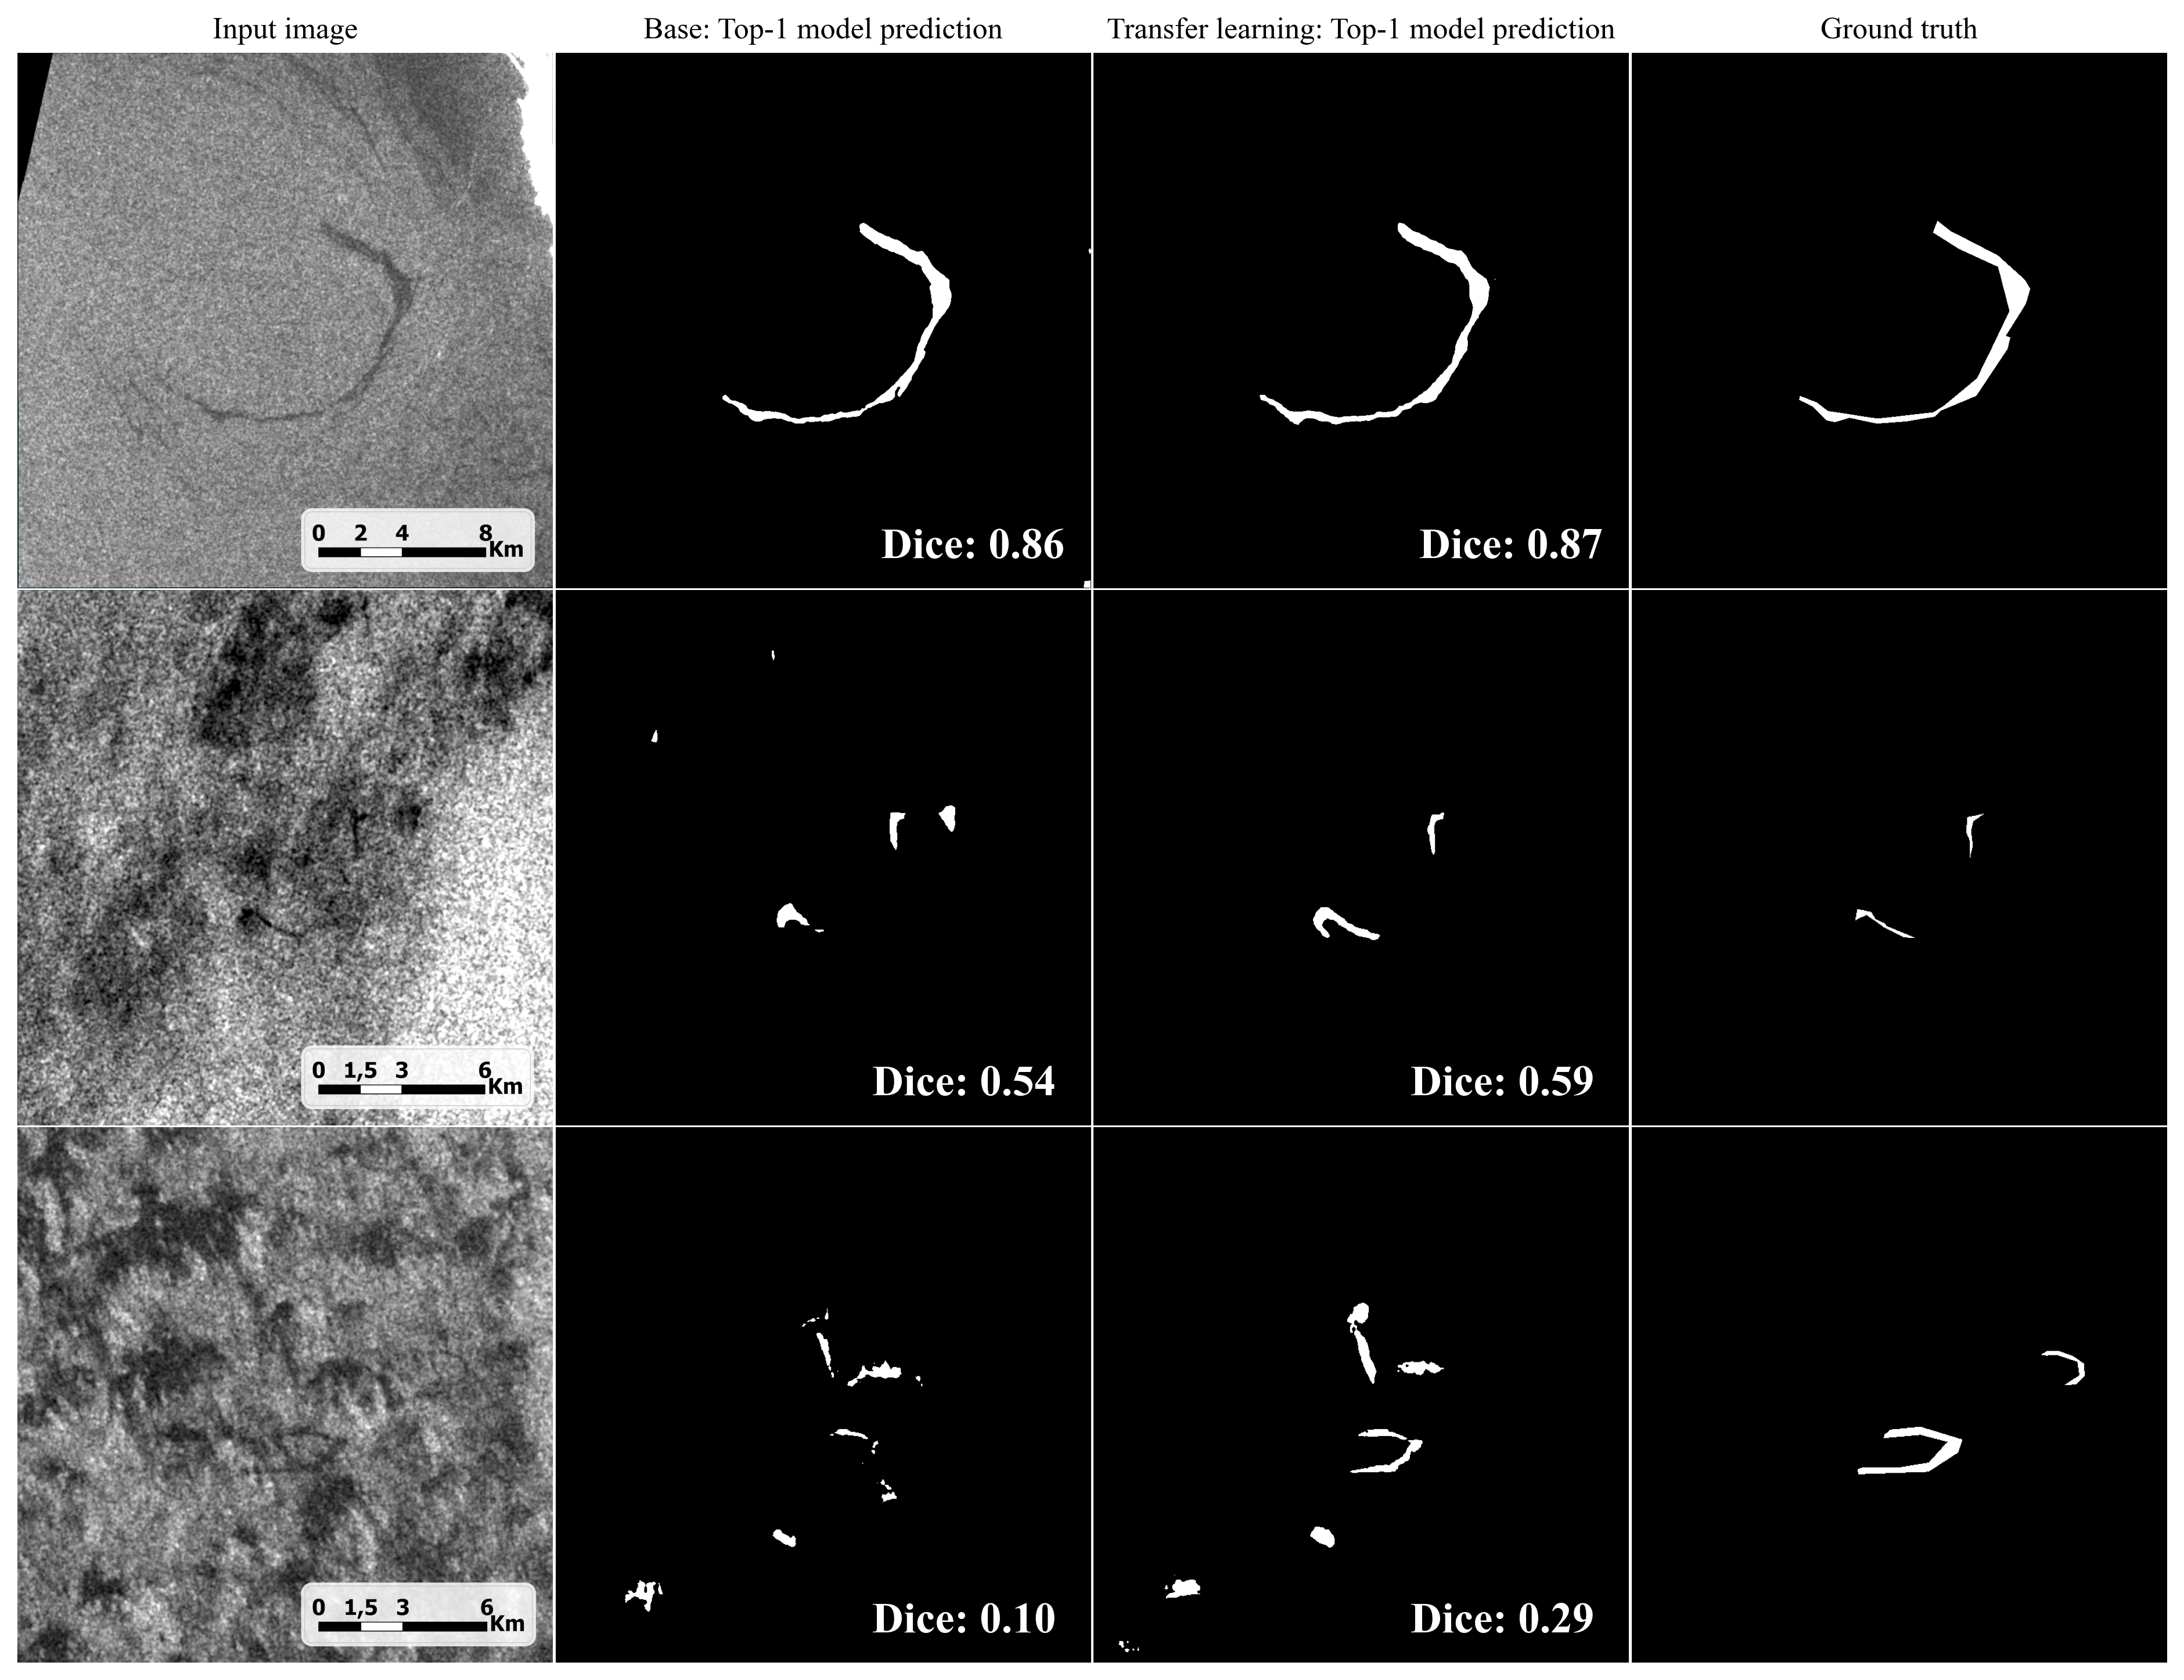
\includegraphics[width=6.2in]{figures/preds4x3_v2_scale.png}
    \caption{Top-1 model performance through examples. \quad Top row: An easier case, with some ocean eddies. \quad Middle: A more challenging example with 
    various look-alike features. \quad Bottom: Arguably one of the most challenging cases. A small, low-contrast slick is missed by models in the center right of the image.}
    \label{figure3}
\end{figure*}
Fig. \ref{figure3} displays the segmentation results predicted from the top-performing model (Top-1). We compare predictions from the base and the fine-tuned
versions, showing how the model benefited from transfer learning accross different contexts. The examples are taken from the test set, with a 25-m resolution and predicting 
with a tile size of 512, the most challenging format evaluated (Table \ref{table2}). In the first row, we see a typical arc-shaped slick in sea conditions allowing a clear SAR damping ratio. 
Both the base and the fine-tuned model delineate the slick while correctly leaving out ocean eddies and a low-wind area on top of the image. The second row presents a common appearance 
of natural slicks in SAR images, where several dark features may trigger false detections. Nonetheless, both models succesfully detect the two slicks and it seems transfer learning help reduce
false positives, despite a somewhat undervalued Dice score. The bottom row examplifies one of the most challenging cases for SAR slick mapping. If two low-contrast slicks can be seen among look-alike features,
only the main one is detected by the fine-tuned model, illustrating the ongoing challenge of mapping under harsh observation conditions. 

\section{Conclusion}
Applications of transfer learning must be carefully evaluated, since in many cases its use can be inefficient, even detrimental if the contexts are too different \cite{mensinkFactorsInfluenceTransfer2022}.
In this study, we made use of labeled slicks originating from a different area and imaged in a different SAR acquisition mode. 
We show that transfer learning in the form of fine-tuning is effective for the few-shot SAR segmentation of natural oil slicks, improving model generalization and reducing overfitting 
despite accessing only a few examples in the target domain.

Image processing to align SAR images is crucial to ensure transferable, high-level features between the source and the target domain—here interferometric-wide (IW) and extra-wide (EW) Sentinel-1 images.
Given these conditions, both deep learning models benefited from transferring pretrained model weights, with DeepLabv3 performing best overall although SAM achieved top accuracy with fewer training images.
The analysis was validated using two documented seeps in the Arctic, where further research could potentially identify additional, undiscovered occurrences. 
Overall, our findings highlight the potential of transfer learning. This approach remains underutilized in remote sensing, yet it is promising for addressing data scarcity, 
with practical applications such as monitoring natural seepage in remote marine environments. 

\section*{Acknowledgments}
Julien Vadnais received financial support from the Doctoral Research Scholarship of the Fonds de recherche du Québec. 
The authors would like to thank the EU Copernicus programme for allowing open access to the Sentinel-1 archives.
\bibliographystyle{IEEEtran}
\bibliography{references}

\end{document}